\documentclass[aps,prb,preprint,superscriptaddress]{revtex4-1}
\usepackage[latin1]{inputenc}	
\usepackage[T1]{fontenc}
\usepackage[cyr]{aeguill}
\usepackage[pdftex]{graphicx}
\usepackage{wrapfig}
\usepackage[english,french]{babel}
\usepackage{amsmath}
\usepackage{amssymb,amsfonts,textcomp}
\usepackage{color}
\usepackage{array}
\usepackage{hhline}
\usepackage{hyperref}
\usepackage{fancyhdr}
\bibliographystyle{unsrt}
\usepackage[pdftex]{graphicx}
\definecolor{violet}{rgb}{0.5,0,0.5}
\definecolor{vert}{rgb}{0,0.65,0}
\definecolor{violet}{rgb}{0.5,0,0.5}
\definecolor{violet2}{rgb}{0.61,0,0.87}
\definecolor{vert}{rgb}{0,0.65,0}
\definecolor{vert2}{rgb}{0,0.6,0}
\definecolor{marron}{rgb}{0.79,0.52,0}
\definecolor{orange}{rgb}{0.87,0.47,0}
\definecolor{lightblue}{rgb}{0,0.8,0.8}
\definecolor{jaune}{rgb}{0.948,0.91,0.17}
\usepackage{ulem}
%\sout{Texte � barrer}
%\xout{Texte � hachurer}
%\uwave{Texte � souligner par une vaguelette}

\begin{document}

%%%%%%%%%%%%%%%%%%%%%%%%%%%%%%%%%%%%%%%%%%%%%%%%%%%%%%%%%%%%%%%%%%%%%%%%%%%%%%%%%%%%%%%%%%%%%%%%%%%%%%%%%%%%%%%%%%%%%%%%%%%%%%%%%%%%%%%%%%%%%%%%%%%%%%
%%%                                                                  TEXTE :                                                                  %%%
%%%%%%%%%%%%%%%%%%%%%%%%%%%%%%%%%%%%%%%%%%%%%%%%%%%%%%%%%%%%%%%%%%%%%%%%%%%%%%%%%%%%%%%%%%%%%%%%%%%%%%%%%%%%%%%%%%%%%%%%%%%%%%%%%%%%%%%%%%%%%%%%%%%%%%

\thispagestyle{empty}
\title{Graphene hybrid near-field optomechanics}

\author{ICFO}
\author{LENS}

\affiliation{Castelldefels, Florence}

\date{\today}
\maketitle

\clearpage
\textbf{abstract.}

%%%%%%%%%%%%%INTRO START%%%%%%%%%%%%%%%%%%%%
\bigskip
%%%%%%%%%%%%%%%%%FIGURE 1 .%%%%%%%%%%%%%%%%%%%%%%%%%%%%
\begin{figure*}[htbp]
\begin{center}
	\includegraphics[width=15cm]{figures/FIGURE1/20150122_FIG1.pdf}
	     \caption{\textbf{Graphene hybrid optomechanical device.}  \textbf{a}: False colour electronic micrograph of a graphene membrane suspended over NVCs embedded in nano-diamonds deposited in holes. \textbf{b}: Confocal reflection (left) and emission (right) spatial maps of a hybrid system. The bright fluorescent spot corresponds to localized emission from NVCs embedded in the nano-diamonds.\textbf{c}: Sketch of the hybrid optomechanical device. The graphene resonator is driven and displaced electrostatically, while its nano-motion is analysed optically.\textbf{d}: Noise spectrum of a graphene resonator at 300K detected by optical interferometry.test}\label{fig:fig1}
\end{center}
\end{figure*}
%%%%%%%%%%%%%%%%%%%%%%%%%%FIGURE 2 :%%%%%%
\begin{figure*}[htbp]
\begin{center}
	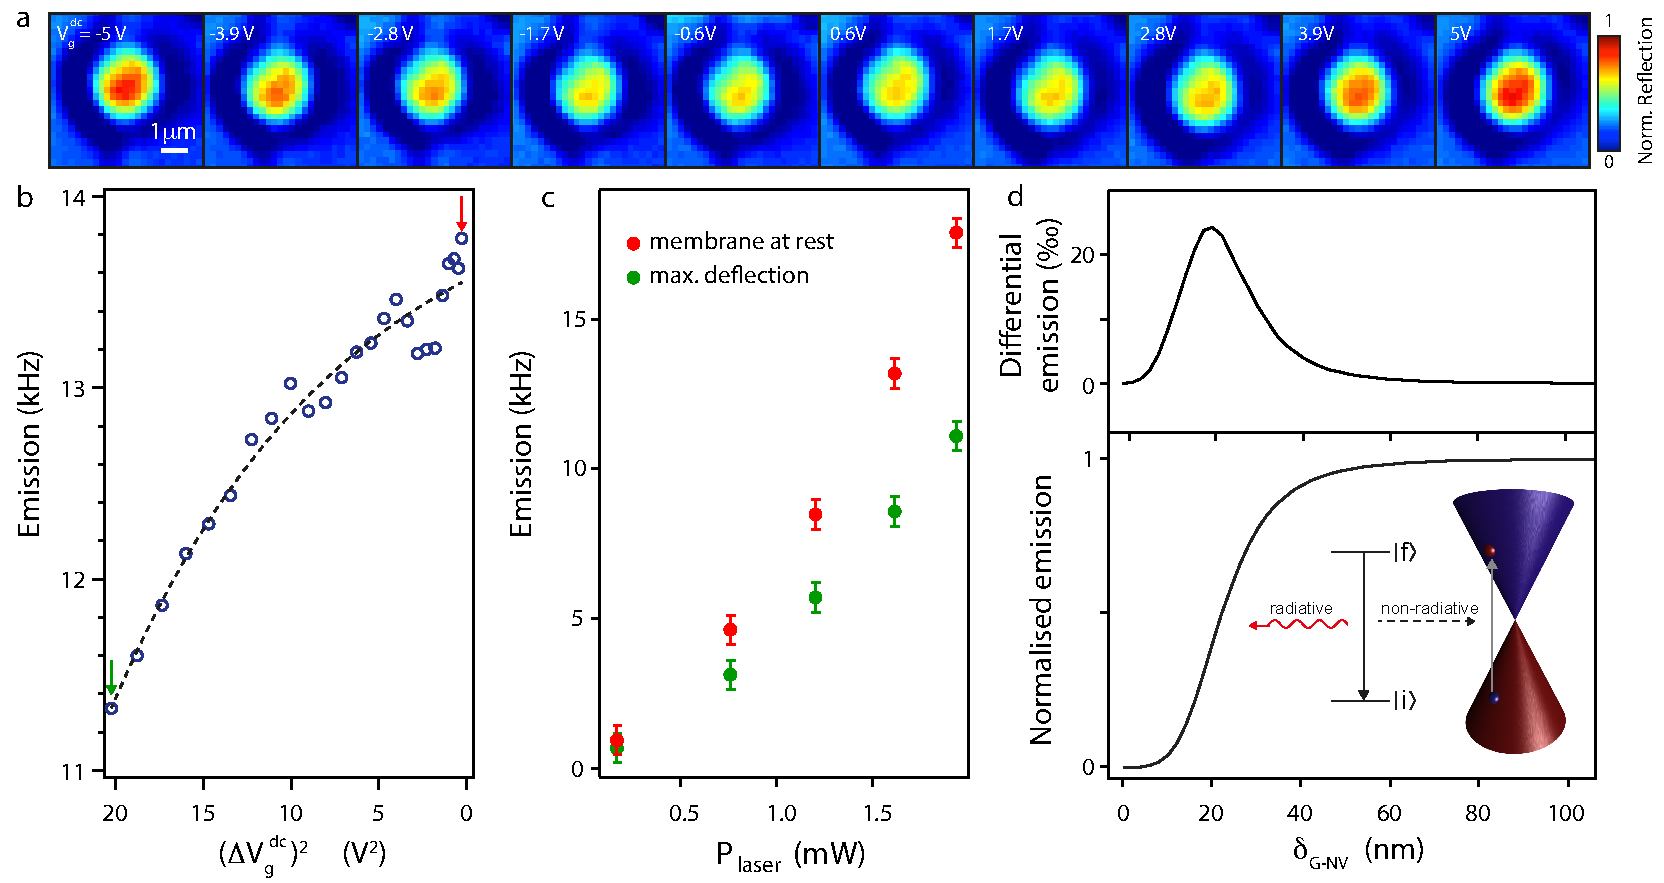
\includegraphics[width=15cm]{figures/FIGURE2/20150122_FIG2.pdf}
	     \caption{\textbf{Coupling of emission to graphene membrane displacement.}  \textbf{a}: Confocal reflection maps of a graphene membrane deflected electrostatically. Each map is recorded at a fixed $\delta_{G-NV}$ given by a static backgate voltage $V_g^{dc}$. The graphene membrane acts as a mobile absorber in the standing wave formed by a single-sided cavity, absorbing a fraction $n_{layer}\pi\alpha I\left ( x,y,\delta_{G-NV}\right )$ at a given point. By electrostatic displacement, the membrane is also warped, leading to a different reflection profile and intensity for a given $V_g^{dc}$. $\delta_{G-NV} \propto \left (\Delta V_g^{dc}\right )^2$. \textbf{b}: NVC emission strength controlled by electrostatic deflection of the membrane. With increasing $\left (\Delta V_g^{dc}\right )^2$, the membrane approaches the NVC, thereby reducing the graphene emitter separation $\delta_{G-NV}$ and quenching the NVC emission. Fitting with eq. 1 allows for calibration of the electrostatic deflection. \textbf{c}: NVC emission versus excitation laser power $P_{laser}$ at two extreme cases of membrane deflection. At rest (\textcolor{red}{$\bullet$}), the power dependence is stronger than at the point of highest deflection (\textcolor{vert}{$\bullet$}) due to enhanced quenching at smaller separations. \textbf{d}: Theoretical dependence of emission (bottom) and differential emission (top) of a single emitter on the distance to a graphene membrane $\delta_{G-NV}$.	Inset : energy diagrams of an optical emitter and graphene at the \textbf{K} point of the Brillouin zone (Dirac cone). For small separations $\delta_{G-NV}< 50$nm, the relaxation of the excited emitter is predominantly non-radiative due to the excitation of electron-hole pairs in graphene.}\label{fig:fig2}
\end{center}
\end{figure*}

Mention Wigner Weisskopf theory : coupling TLS with continuum.
%%%%%%%%%%%%%%%%%%%%%%%FIGURE 3:.%%%%%%%%%%%%%%%%%%%%%%%%%%%
\begin{figure*}[htbp]
\begin{center}
		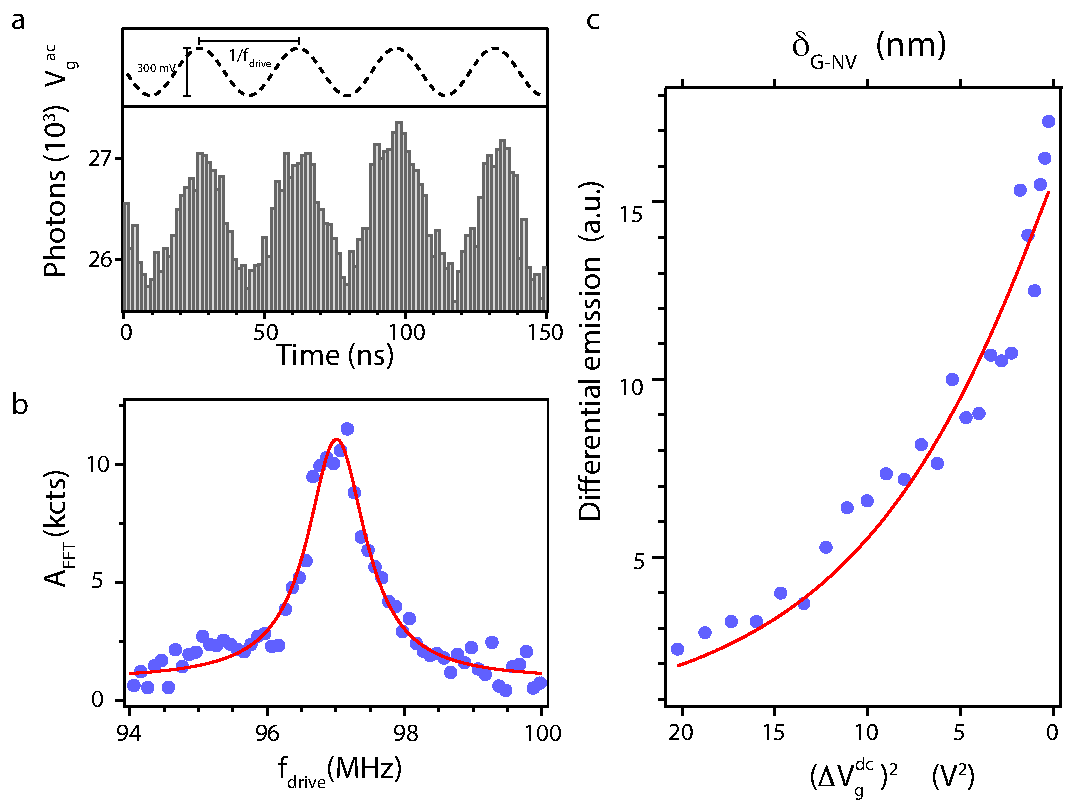
\includegraphics[width=16cm]{figures/FIGURE3/20150122_FIG3.pdf}
	     \caption{\textbf{Readout of graphene nano-motion via NVC emission.} \textbf{a}: Time trace of NVC emission (grey bars) modulated by a driven graphene membrane oscillating in its near field. Distance-dependent  quenching imprints the nano-motion of the graphene membrane onto the emission. \textbf{b}: Mechanical resonance obtained from differential NVC emission. Each point corresponds to the amplitude of the Fourier component at $f=f_{drive}$ of the emission time trace (as in \textbf{a}). A Lorentzian fit of the data (red line) yields the same value for $f_m$ as obtained independently by optical interferometry. \textbf{c}: Differential emission (blue) as a function of $\left ( \Delta V_g^{dc}\right )^2$, normalised by the oscillation amplitude $A_m$ of the membrane at resonance.}\label{fig:fig3}
\end{center}
\end{figure*}

%%%%%%%%%%%%%%%%PERSPECTIVES + CONCLUSION %%%%%%%%%%%%%%%%%%%%%%%%%


\end{document}
